\section{La programmation orientée objet}
\begin{frame}
	\begin{center}
	\huge
	La programmation orientée objet
	\end{center}
\end{frame}

\subsection{Notion d'objet} %%%%%%%%%%%%%%%%%%%%%%%%%%%%%%%%%%%%%%%%%
\begin{frame}
	\frametitle{Comme une boite}
	\begin{center}
	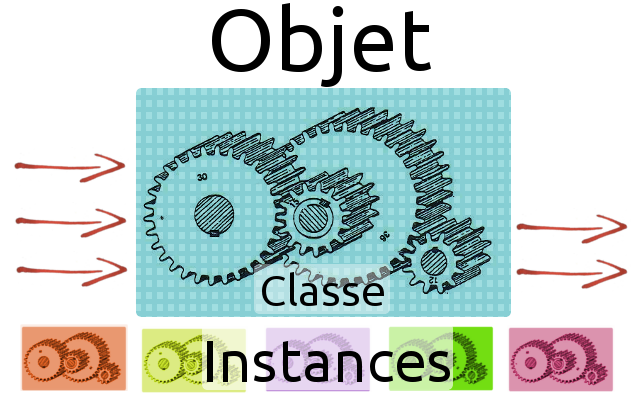
\includegraphics[width=9cm]{pics/explObj1.png}
	\end{center}
\end{frame}
\begin{frame}
	\frametitle{Attributs/Méthodes}
	\begin{center}
	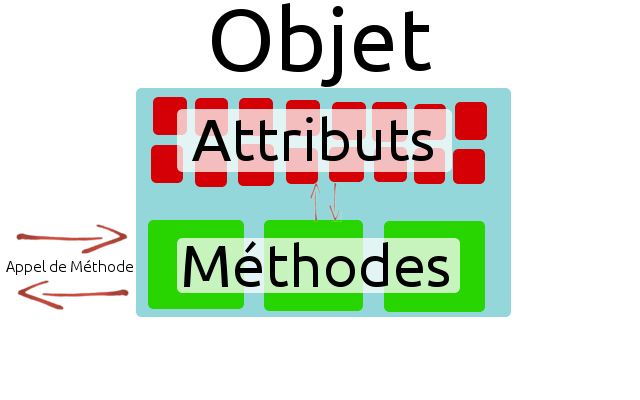
\includegraphics[width=9cm]{pics/explObj2.png}
	\end{center}
\end{frame}
\begin{frame}[fragile]
	\frametitle{Exemple d'utilisation d'objet}
	\begin{lstlisting}
let (c1,c2) =
  let m1 = new CoffeeMachine(Bresile)
  and m2 = new CoffeeMachine(Islande)
  in
  m1#addWater(1000);
  m2#addWater(42000);
  m1#headUp();
  m2#headUp();
  (m1#getCoffee(1),m2#getCoffee(3))
;;
	\end{lstlisting}
\end{frame}

\subsection{La déclaration d'un objet} %%%%%%%%%%%%%%%%%%%%%%%%%%%%%%
\begin{frame}[fragile]
	\frametitle{Syntaxe}
	\begin{minipage}{0.45\textwidth}
		\lstset{basicstyle=\small}
		\begin{lstlisting}
class name parameters =
  object
    (*Attributes*)
    
    (*Methods*)
  end
		\end{lstlisting}
	\end{minipage}
	\begin{minipage}{0.4\textwidth}
		\begin{lstlisting}
class point x y =
  object
    val x = x
    val y = y

    method printCoord =
      print_int x;
      print_string ",";
      print_int y;
      print_string "\n"
  end
		\end{lstlisting}
	\end{minipage}
\end{frame}

\begin{frame}[fragile]
	\frametitle{Déclaration d'attribut}
	\textit{Utilisez un type explicite pour les méthodes (pas de polymorphisme, pour l'instant...).}\\
	\begin{block}{Simple}
		\begin{lstlisting}
  val name = expr
		\end{lstlisting}
	\end{block}
	\begin{block}{Modifiable}
		\begin{lstlisting}
  val mutable name = expr
  name <- expr
		\end{lstlisting}
	\end{block}
	\begin{block}{Lorsque rien ne marche : Le type Option}
		\begin{lstlisting}
  val mutable name = None
  name <- Some expr
		\end{lstlisting}
	\end{block}
\end{frame}

\begin{frame}[fragile]
	\frametitle{Déclaration de méthode}
	\begin{block}{Public}
		\begin{lstlisting}
  method name parameters = expr
		\end{lstlisting}
	\end{block}
	\begin{block}{Privée}
		\begin{minipage}{0.4\textwidth}
  			\begin{lstlisting}
  class name =
    object
    ...
    end
			\end{lstlisting}
		\end{minipage}$\Rightarrow$
		\begin{minipage}{0.4\textwidth}
			\begin{lstlisting}
  class name =
    object (self)
    ...
    end
			\end{lstlisting}
		\end{minipage}
	\end{block}
	\begin{lstlisting}
  method private name parameters = expr
  self#privateMethod parameters
	\end{lstlisting}
\end{frame}

\begin{frame}[fragile]
	\frametitle{Initialisation}
	\begin{lstlisting}
class putListInQueue (l:int list) =
  object (self)
    
  val data = Stack.create ()

  initializer
    let rec storage = function
      | [] -> ()
      | e::q -> 
        push e data;
        storage q
    in storage l

  ...
  end
	\end{lstlisting}
\end{frame}

\begin{frame}[fragile]
	\frametitle{Attributs polymorphiques}
	\begin{lstlisting}
class ['a] name parameters =
  object 
  val data = ref []

  method add (e:'a) =
    data := e::!data
  
  ...
  end
	\end{lstlisting}
\end{frame}

\subsection{L'héritage} %%%%%%%%%%%%%%%%%%%%%%%%%%%%%%%%%%%%%%%%%%%%%
\begin{frame}[fragile]
	\frametitle{Syntaxe de l'héritage}
	\begin{lstlisting}
class childName parameters =
  object
  inherit motherClass mothersParameters

  end
	\end{lstlisting}
	\begin{lstlisting}
class childName parameters =
  object
  inherit motherClass mothersParameters 
    as motherSuper

  end
	\end{lstlisting}
\end{frame}

\begin{frame}
	\frametitle{Accès aux méthodes de la classe mère 1/2}
	\lstinputlisting[firstline=1, lastline=14]{code/heritage.ml}
\end{frame}

\begin{frame}
	\frametitle{Accès aux méthodes de la classe mère 2/2}
	\textit{Le type d'une réécritrue d'une méthode doit correspondre à celui de la méthode mère.}
	\lstinputlisting[firstline=16, lastline=28]{code/heritage.ml}
\end{frame}
\subsection{Le polymorphisme de sous-type} %%%%%%%%%%%%%%%%%%%%%%%%%%%
\begin{frame}
	\frametitle{Le polymorphisme de sous-type}
	\begin{center}
		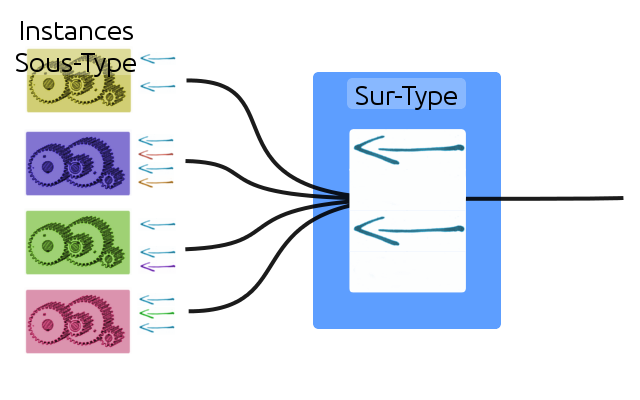
\includegraphics[width=9cm]{pics/inclusionObjet.png}
	\end{center}
\end{frame}

\begin{frame}[fragile]
	\frametitle{Interface et opérateur de sous-type}
	\framesubtitle{L'interface}
	\textit{On peut utiliser une classe ou une interface pour faire du polymorphisme de sous-type.}
	\begin{block}{Opérateur}
		~~Instance\_Sous-Type \large{:>} Sur-type
	\end{block}
	\begin{block}{Interface}
		\begin{lstlisting}
  class type interfaceName =
    object
      method mInterface1 : type1
      method mInferface2 : type2
    end
		\end{lstlisting}
	\end{block}
	\textit{Les types des méthodes doivent correspondre à ceux des méthodes de l'interface/classe.}
\end{frame}

\begin{frame}[fragile]
	\frametitle{Interface et opérateur de sous-type}
	\framesubtitle{Exemple d'utilisation}
	Réutilisons les class point et colored\_point.
	\begin{lstlisting}
let f (o:point) = o#setCoord 4 2
let test = 
  ((new colored_point (4,2) 255):>point)

test#print;
f test;
test#print;
test#setData 4 5 1
	\end{lstlisting}
	\begin{block}{Sortie}
		\begin{lstlisting}
  (2,4) 255
  (4,2) 255
  Error: This expression has type point
         It has no method setData
		\end{lstlisting}
	\end{block}
\end{frame}
